\newpage
\appendix
\section{Appendix}\label{sec:appendix}

\subsection{Uncertainties}\label{sec:uncertainties}
%TODO Übersetzung

Alle Unsicherheiten werden nach dem GUM bestimmt und berechnet.
Die Gleichungen dazu finden sich in \ref{fig:GUM_combine} und \ref{fig:GUM_formula}.
Hierfür wurde die Python Bibliothek \enquote{uncertainties} verwendet, welche den Richtlinien des GUM folgt.
Für die Unsicherheiten der Parameter in Annäherungskurven wurden die $y$-Unsicherheiten der anzunähernden Werte beachtet und die Methode der kleinsten Quadrate angewandt.
Dafür steht in der Bibliothek die Methode \enquote{scipy.optimize.curve\_fit()} zur Verfügung.

Für Messungen mit digitalen Anzeigen wird eine rechteckige Verteilung mit $\sigma_X = \frac{\Delta X}{2\sqrt{3}}$ aufgrund der begrenzten Ziffernzahl und für analoges Ablesen wird eine Dreiecksverteilung mit $\sigma_X = \frac{\Delta X}{2\sqrt{6}}$ angenommen.
Die jeweiligen $\Delta X$ sind im entsprechenden Abschnitt zu finden.

\begin{figure}[ht]
	\begin{equation*}
	x = \sum_{i=1}^{N} x_i
	;\quad
	\sigma_x = \sqrt{\sum_{i = 1}^{N} \sigma_{x_i}^2}
	\end{equation*}
	\caption{Formel für kombinierte Unsicherheiten des selben Typs nach GUM.}
	\label{fig:GUM_combine}
\end{figure}

\begin{figure}[ht]
	\begin{align*}
	f = f(x_1, \dots , x_N)
	;\quad
	\sigma_f = \sqrt{\sum_{i = 1}^{N}\left(\pdv{f}{x_i} \sigma_{x_i}\right) ^2}
	\end{align*}
	\caption{Formel für sich fortpflanzende Unsicherheiten erster Ordnung nach GUM.}
	\label{fig:GUM_formula}
\end{figure}

%\newpage
%\subsection{weitere Abbildungen}

\subsection{SPEs additional figures}
\label{sec:anhang:spe}

\begin{figure}[!ht]
    \centering
    \begin{subfigure}{0.47\textwidth}
        \centering
        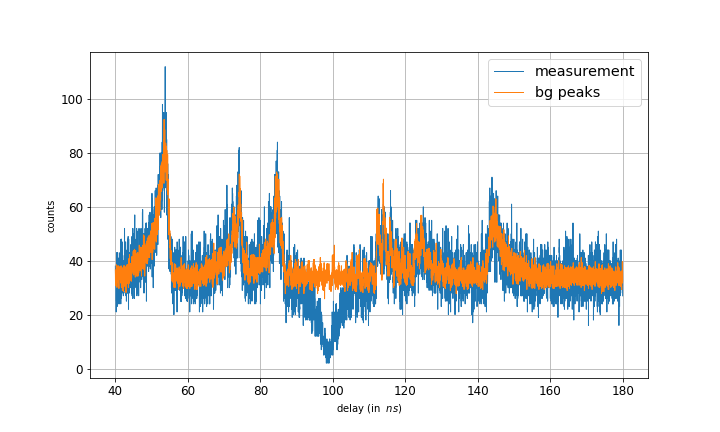
\includegraphics[width=1.0\textwidth]{img/output_t2/50.0muW_bg_peaks.png}
    		\caption{}
    		%\label{fig_antibunch_background_comp}
    \end{subfigure}
    %\hfill
    \begin{subfigure}{0.47\textwidth}
        \centering
        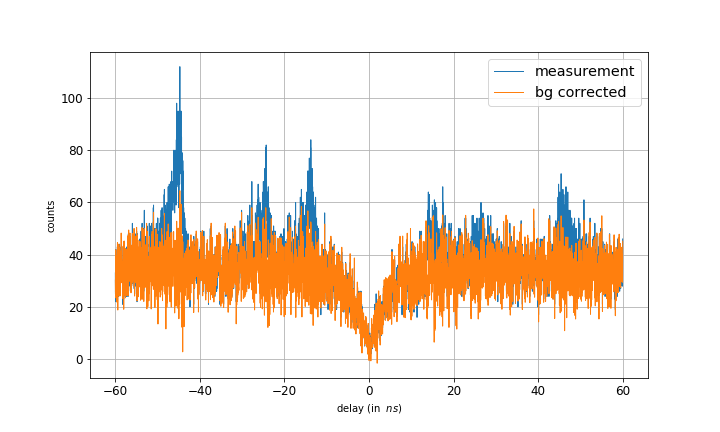
\includegraphics[width=\textwidth]{img/output_t2/50.0muW_bg_vgl.png}
        \caption{}
        %\label{fig_antibunch_raw_corr_comp}
    \end{subfigure}
    \caption{a: Antibunching measurement as recorded and compared to the adjusted background signal. b: Antibunching measurement as recorded and compared to the background corrected signal. The laser power is \SI{50}{\micro W}.} %hoffe ok, dass der eine so doppelt ist
	%\label{fig_antibunch_comp}
\end{figure}
\begin{figure}[!ht]
    \centering
    \begin{subfigure}{0.47\textwidth}
        \centering
        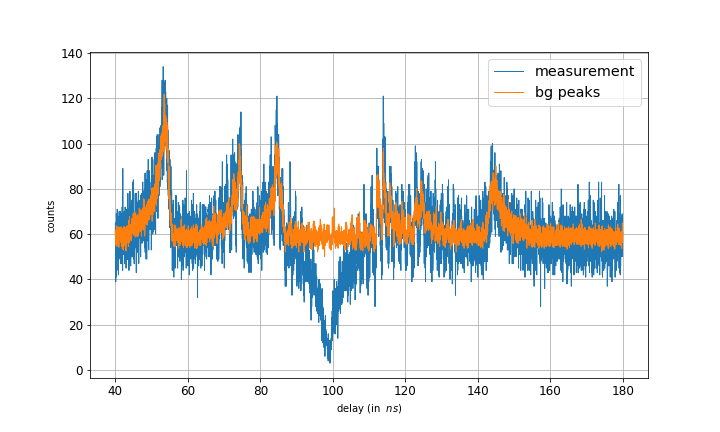
\includegraphics[width=1.0\textwidth]{img/output_t2/100.0muW_bg_peaks.png}
    \caption{}
    %label{fig_antibunch_background_comp}
    \end{subfigure}
    %\hfill
    \begin{subfigure}{0.47\textwidth}
        \centering
        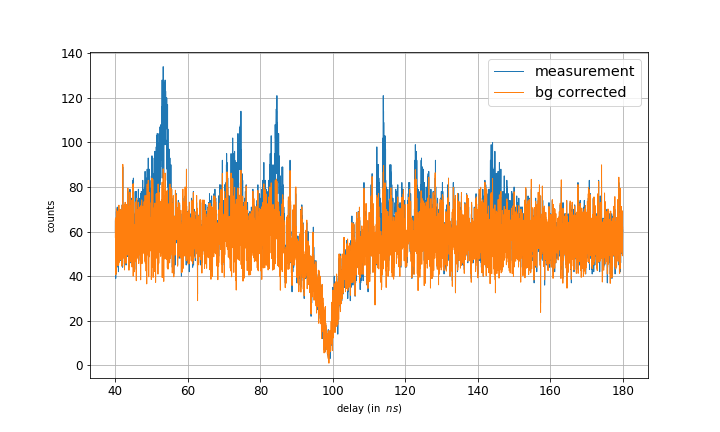
\includegraphics[width=\textwidth]{img/output_t2/100.0muW_bg_vgl.png}
        \caption{}
        %label{fig_antibunch_raw_corr_comp}
    \end{subfigure}
    \caption{a: Antibunching measurement as recorded and compared to the adjusted background signal. b: Antibunching measurement as recorded and compared to the background corrected signal. The laser power is \SI{100}{\micro W}.} %hoffe ok, dass der eine so doppelt ist
	%label{fig_antibunch_comp}
\end{figure}
\begin{figure}[!ht]
    \centering
    \begin{subfigure}{0.47\textwidth}
        \centering
        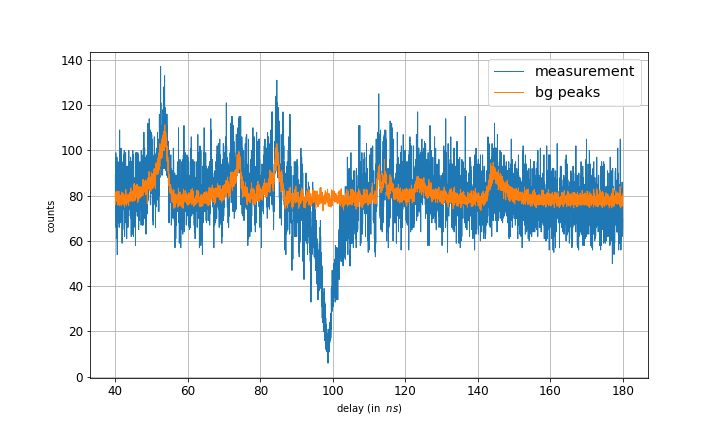
\includegraphics[width=1.0\textwidth]{img/output_t2/250.0muW_bg_peaks.png}
    \caption{}
    %label{fig_antibunch_background_comp}
    \end{subfigure}
    %\hfill
    \begin{subfigure}{0.47\textwidth}
        \centering
        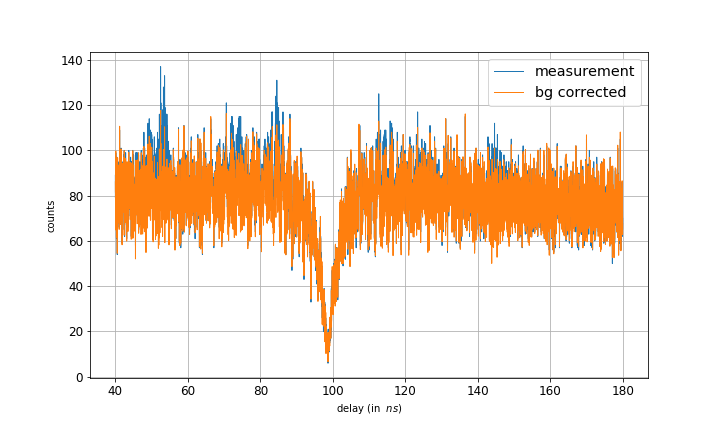
\includegraphics[width=\textwidth]{img/output_t2/250.0muW_bg_vgl.png}
        \caption{}
        %label{fig_antibunch_raw_corr_comp}
    \end{subfigure}
    \caption{a: Antibunching measurement as recorded and compared to the adjusted background signal. b: Antibunching measurement as recorded and compared to the background corrected signal. The laser power is \SI{250}{\micro W}.} %hoffe ok, dass der eine so doppelt ist
	%label{fig_antibunch_comp}
\end{figure}
\begin{figure}[!ht]
    \centering
    \begin{subfigure}{0.47\textwidth}
        \centering
        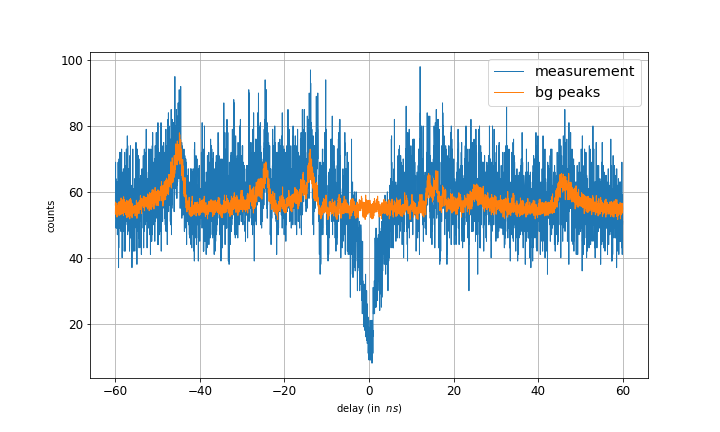
\includegraphics[width=1.0\textwidth]{img/output_t2/500.0muW_bg_peaks.png}
    \caption{}
    %label{fig_antibunch_background_comp}
    \end{subfigure}
    %\hfill
    \begin{subfigure}{0.47\textwidth}
        \centering
        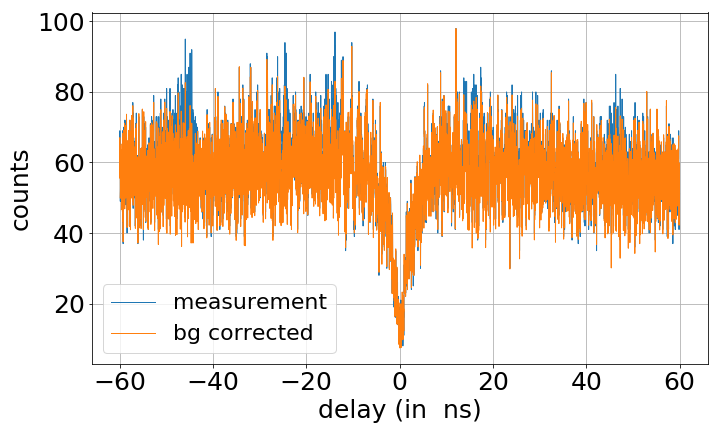
\includegraphics[width=\textwidth]{img/output_t2/500.0muW_bg_vgl.png}
        \caption{}
        %label{fig_antibunch_raw_corr_comp}
    \end{subfigure}
    \caption{a: Antibunching measurement as recorded and compared to the adjusted background signal. b: Antibunching measurement as recorded and compared to the background corrected signal. The laser power is \SI{500}{\micro W}.} %hoffe ok, dass der eine so doppelt ist
	%label{fig_antibunch_comp}
\end{figure}
\begin{figure}[!ht]
    \centering
    \begin{subfigure}{0.47\textwidth}
        \centering
        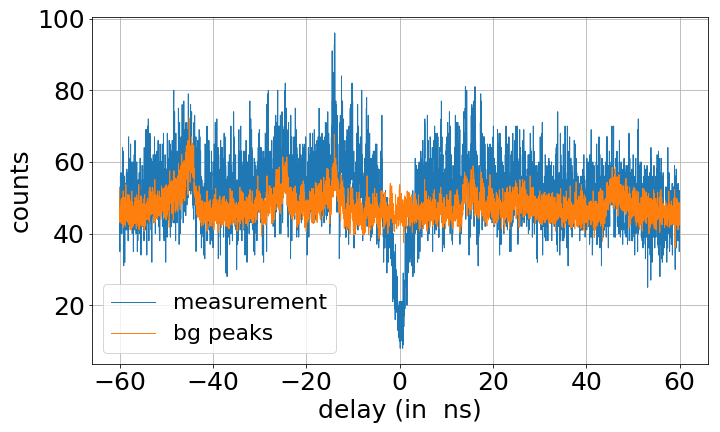
\includegraphics[width=1.0\textwidth]{img/output_t2/1000.0muW_bg_peaks.png}
    \caption{}
    %label{fig_antibunch_background_comp}
    \end{subfigure}
    %\hfill
    \begin{subfigure}{0.47\textwidth}
        \centering
        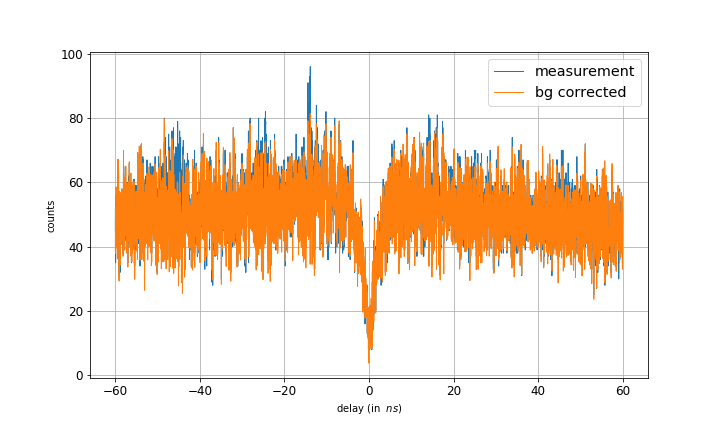
\includegraphics[width=\textwidth]{img/output_t2/1000.0muW_bg_vgl.png}
        \caption{}
        %label{fig_antibunch_raw_corr_comp}
    \end{subfigure}
    \caption{a: Antibunching measurement as recorded and compared to the adjusted background signal. b: Antibunching measurement as recorded and compared to the background corrected signal. The laser power is \SI{1000}{\micro W}.} %hoffe ok, dass der eine so doppelt ist
	%label{fig_antibunch_comp}
\end{figure}
\begin{figure}[!ht]
    \centering
    \begin{subfigure}{0.47\textwidth}
        \centering
        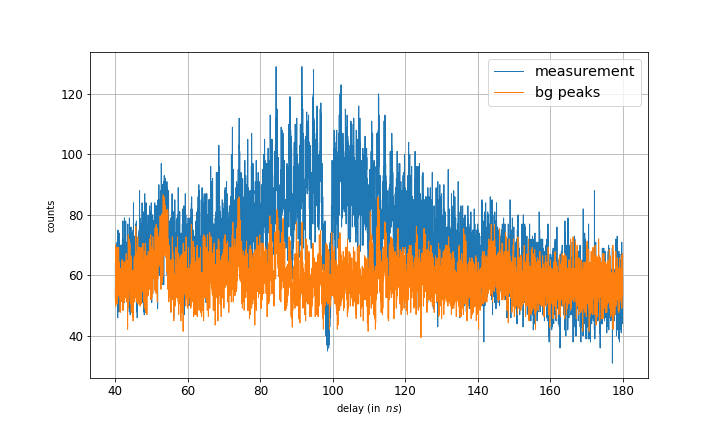
\includegraphics[width=1.0\textwidth]{img/output_t2/2000.0muW_bg_peaks.png}
    \caption{}
    %label{fig_antibunch_background_comp}
    \end{subfigure}
    %\hfill
    \begin{subfigure}{0.47\textwidth}
        \centering
        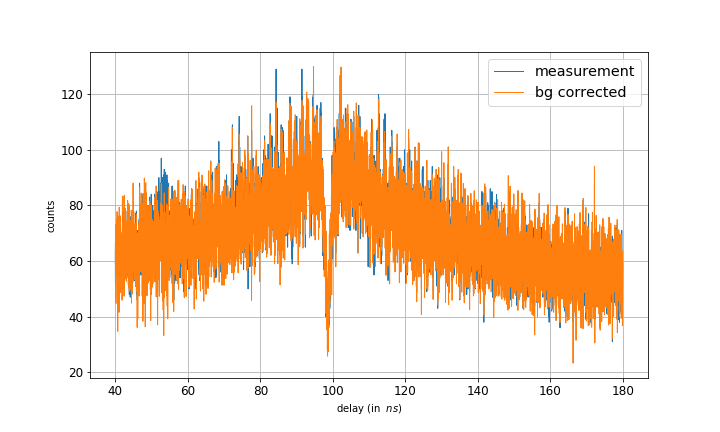
\includegraphics[width=\textwidth]{img/output_t2/2000.0muW_bg_vgl.png}
        \caption{}
        %label{fig_antibunch_raw_corr_comp}
    \end{subfigure}
    \caption{a: Antibunching measurement as recorded and compared to the adjusted background signal. b: Antibunching measurement as recorded and compared to the background corrected signal. The laser power is \SI{2000}{\micro W}.} %hoffe ok, dass der eine so doppelt ist
	%label{fig_antibunch_comp}
\end{figure}
